\section{Automating Metadata Acquisition}
%
%-building names dirty -> we need some way to characterize them
%-learn
%-input output example
%-who will generate these - maybe building manager, maybe users
%-ease of use as opposed to people writing regular expressoin themselves.
%-why not have someone write the regex expressions for those most common sensors ? because people who know are not the people who use the data. building managers know, people working closely with a sensor deployment know. Sometimes the regex might get complex ...... for instanct, when is a particular tag applicable ? 
%
%Why is it this way ?

In this section, we go into detail about how we apply program synthesis techniques and the input-output model of interaction to extract enough information from sensor names to enable sufficient coverage of sensor applications. We first provide a  general overview of the technique in Section~\ref{}, followed by details of the input required, the synthesis algorithm in Section~\ref{}. 

%As explained earlier, most sensor names ( or SCADA\footnote{Supervisory Control and Data Acquisition} tags ) try to encode some level of semantic information. These names might have been generated by the individual who was in charge of commissioning a building, or by following a set of vendor-specific rules. In either case, the encoded sensor names convey very little meaning to people who are not familiar with the building layout.
%
%A lot of the sense points contained in a particular building is very site-specific, e.g a building may contain a fault detector for its backup chiller, for which there might not be a well-defined sensor labelling schema from the vendor. In such scenarios, the agent commissioning a building tries his best to convey the information by using indicative labels. E.g we encountered points labelled \texttt{BLDA4S18SASA\_M}, which denotes an alarm if the supply air temperature setpoint for a supply fan gets too high\footnote{The point is to be read thus : the building name is denoted by {\it BLD}, {\it A4} indicates an air handling unit whose identification number if $4$. {\it S$18$} denotes a supple fan whose identification number if $18$, and {\it SASA\_M} denotes a supply alarm setpoint}. 
{\bf Terminology :} We shall refer to each distinct component of a sensor name, which together signify some semantic content as a label. For instance, the example mentioned in the previous section \texttt{BLDA1R435\_\_ART} has six labels --- \texttt{BLD, A, 1, R, 435} and \texttt{ART}. A \emph{tag} qualifies the label to a standard namespace. In our example,  

\subsection{Algorithm Overview}ope
The main aim of this algorithm is to learn the regular expressions that identify different labels in a sensor name. We require an expert to give examples on how to resolve label boundaries for a particular sensor name, and the metadata tag that qualifies it. The algorithm generates a wide set of regular expressions which could extract the given label from the sensor name. When another example containing the same labels is given by the expert, the algorithm intersects the set of regular expressions obtained from the two examples, and developes and classifier which identifies which sensor names contains that particular label. As more examples are added, the classifier gets tuned and so does the regular expression needed to find a label. 

some intro into what we are doing to automate



\subsection{final output - project Haystack}

final output maybe in any form. 
we realized going into this soon that not all tags conformed to any known schema. 
For the general tags like room, ahu, vav we have conformed to the project haystack ones. 
for the remainder of the points which are building specific, we just require that a person uses a consistent schema. 


Boosting the metadata can enable better usability across buildings. The question automatically becomes which metadata space to normalize to. There are many metadata schemes devised for representing all buildings. Some of them are too specific and require heavy lifting, and some of them are too simple and do not meet the criteria of being expressive enough for the necessary facets of a building. 


The goal is to normalize the existing metadata. 

\subsection{ formalize what we want as output from a string token}

what is the input ? 
well the input is 



- the model is we present the user an example to classify
- the expert goes in and classified every tag he knows in the building. he can see the list of tags in the building while doing so. 
- the user also tells us which position each string corresponds to 
- whether a value is a constant or a variable.

\subsection{techniques - learning from example}

There is a lot of related work in obtaining structured data from unstructured data formats. 

1. learning by example
2. data wrangler

-the core idea is to generate as many possible regular expressions as possible and then slowly refine our model as we get more and more examples.



\subsection{Technique Overview}

The synthesis technique is adapted from ~\cite{gulwani}, and tries to learn the regular expressions which 

of our technique is to provide building-specific experts the ability to come up with ur technique tried to learn the regular expression patterns that 
\subsection{learning by example}

-The basic structure of our technique is derived from gluwani.
-The goal is to 

Our proposed technique is derived from the synthesis technique developed in ~\cite{}. In this section, we provide an overview of the technique, and then we will introduce how we adapt this technique to our problem. 

At a very high level, the algorithm tries to compute all possible transformations that can transform an input string to an output string. The possibilities include a {\it Substring(i,j)} operation or simple position matching operation {\it{CPos}}. The two indices in the substring operation can be obtained by a regular expression, where the regular expression is  



 way we learn regular expressions from inputs provided by the expert. We shall use the example scada tag {\tt BLDA1R465  ART} as a goto example throughout this section.

In the following sections, we will use the word {\it token} to refer a token from a character class. So a token might be is a character or a group of characters in a point to be expanded. In the For instance, in the point {\tt BLDA1R465 ART} has the tokens as shown in Figure~\ref{fig:exampleInput}


\subsubsection{Inputs}

For every example an expert provides, we require three types of information - (a) the normalized metadata tag which is contained in the point name,  (b) the mapping of the labels in the data to normalized metadata tags , (c) the starting point of those labels, and (d) whether the value of the label is a constant or variable. For instance, consider the expert is asked to fully qualify the sensor point name \texttt{BLDA1R435\_\_ART}. Shown below is the expected input by the user.

\begin{figure}[h!]
  
  \centering
    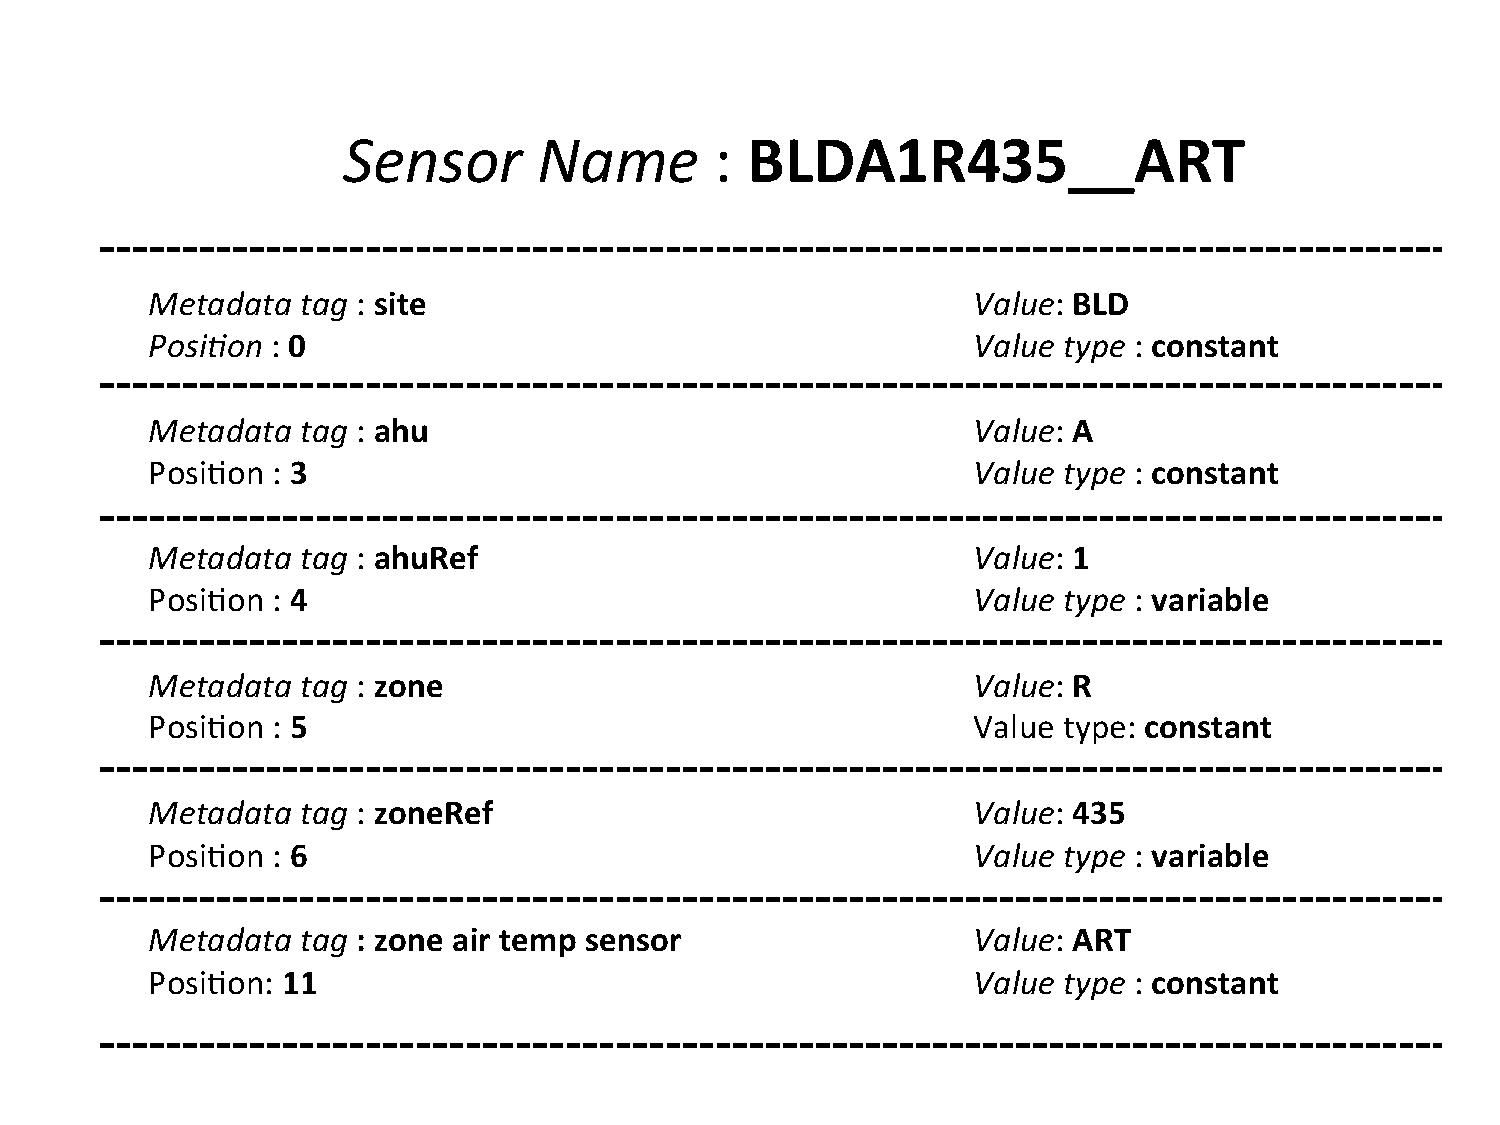
\includegraphics[width=0.5\textwidth]{figs/inputExample.pdf}
\caption{Input provided by the expert for fully qualifying the semantic structure of a sensor point name}
\label{fig:exampleInput}
\end{figure}

The aim of the learning algorithm would then be to fully qualify the remaining examples



Whenever the expert types in the explanation for an input, we require that the expert give a full description of the point. The full description of a point consist of the haystack tags the point contains, the starting and ending position of the string that correspond to the haystack tag, mentioning whether the substring is a constant or is variable. For instance, in our example, {\tt BLD} is a constant for the haystack tag {\bf site}, but {\tt 465} is a variable substring, because the tag value will change from point to point. 


are the tokens contained in a tag, their starting and ending positions, whether the tag has an associated value, and whether the associated value 

\subsection{challenges}


-different types of points all together in the same corpus, and it is not one or two . you have to generate a regex classifier for all known tags. 
-tokens vary from building to building -> so no pre-defined token ( alternative were using Excel's stuff or treating every letter as an individual token ). Show the experiment that shows the number of incorrectly qualified vs number of examples added.
-simplest classifier to more complex classifier



\subsection{technique we chose and modifications}

learning by input output example
- subtring generation
-intersection
-predicate generation

\begin{figure}[h!]
  
  \centering
    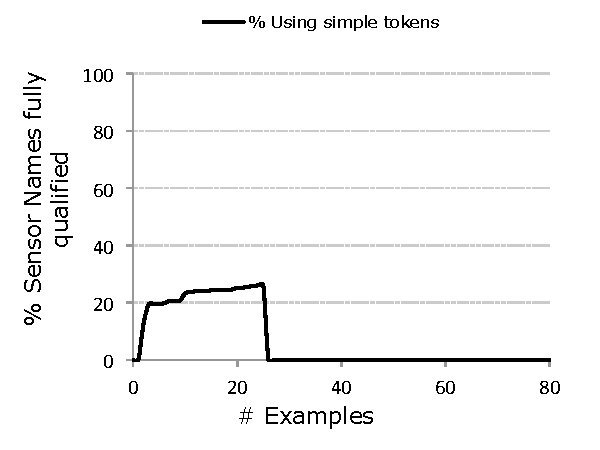
\includegraphics[width=0.5\textwidth]{figs/gulwani-noconverge.pdf}
\caption{Number of sensor names fully qualified with a token set consisting simply of alphabetic characters [A-Z], numerals [0-9], and one token for each special character.}
\label{fig:simpleTokenNoCoverage}
\end{figure}


\section{Evaluation of Learning By Example}

In this section, we guage the effectiveness of our learning by example technique by evaluating the number of examples required to qualify labels in two large commercial buildings. 

\subsection{Test Buildings for Evaluation}

We manually generated ground truth data for all the points in two buildings whose building management system was installed by different vendors. Building $1$ has 1586 sensor points and was built in the 1990s. Building $2$ was built in the 2000s and has 2551 sense points. The label characteristics of the two buildings are shown in Figure~\ref{fig:buildingLabelCharacteristics}. 

Figure~\ref{fig:labelFreq} shows that in  these two buildings, a few labels (about 20 in each building) frequently appear in a lot of sensor names. This is pretty common in commercial buildings, where a majority of the points are related to zone or room information. For instance, Building $1$, has a room setpoint sensor, an airflow sensor and temperature sensor for each of its more than 200 rooms. Each of these points have a label indicating that they are a room, and a room number. These most frequent labels also fully qualify a large number of the sensor names in both buildings. In other words, learning proper classifiers and qualifications for about 20 labels could yield a full qualification for 80\% of the sensor names in both these buildings.

The distribution frequency of labels also has a long tail. For both the buildings, the labels corresponding to {\it site} and {\it zoneRef} are most common. However, the distribution of labels show that there is also a long tail. These comprise of building specific sensors, alarms or status variables. There are also a lot of incomplete or inconsistent labeling of sensor names, the labels of which fall in this long tail. Thus, one of the main objectives of the learning algorithm is that it does not learn wrong classifiers for labels based on sensor names that fall in this long tail.

\begin{figure}[h!]]
\centering
	\begin{subfigure}{0.48\textwidth}
                \centering
		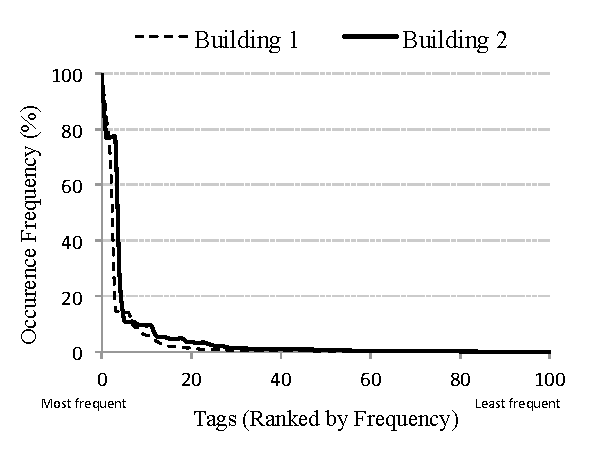
\includegraphics[width=\textwidth]{./figs/pointOccuranceFreq.pdf}
                \caption{Percentage of sensor names each label appears in. The x-axis is sorted according to the frequency of occurence of a label}
                \label{fig:labelFreq}
	\end{subfigure}
	\begin{subfigure}{0.48\textwidth}
                \centering
		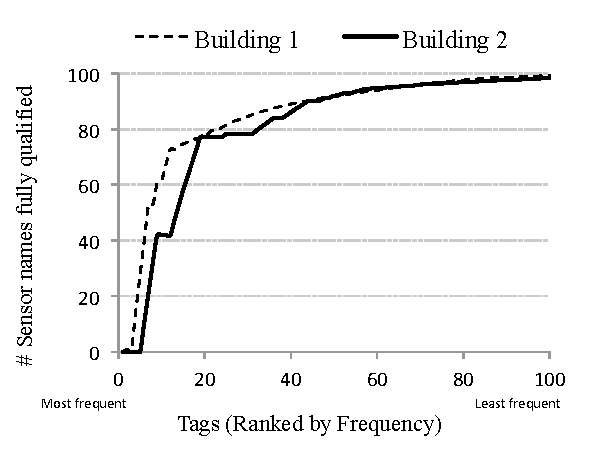
\includegraphics[width=\textwidth]{./figs/pointCDF.pdf}
                \caption{Percentage of sensor names fully qualified by the highest ranking labels. A point ($x$,$y$) indicates that $y$ sensor names could be fully qualified by using labels ranked $1$ ... $x$}
                \label{fig:pointCDF}
	\end{subfigure}
\caption{Characteristics of labels from two buildings we generated ground-truth data to test our learning technique}
\label{fig:buildingLabelCharacteristics}
\end{figure}



\subsection{Convergence of labels}





\subsection{Choosing the Next Example}


The large number of sensors in a building pose a challenge in selecting the next example to present to the expert. First, the expert might not always be able to browse through all sensor points to check correct qualification. Also, an expert might visally not be able to discern which points would add the most amount of information to the learning process. 

This process can be facilitated by the internal notion the learning algorithm has of how much of each sensor name it has been able to qualify. This notion is maintained by simply comparing the sensor name to all the labels that the algorithm applied on it. Note that, the algorithm can incorrectly apply labels on a sensor name, which may lead to erroneous conclusions. The incorrect application of labels might be due to incorrectness or incompleteness of the boolean matching expression or the string extraction regular expressions.

We implemented four different generators to evaluate which example should be provided next to the expert:

{\bf Random:} This generator just finds at random the next example to present to the expert. While choosing the example, the random algorithm chooses among the set of sensor names which it feels it has not been able to fully qualify.  

{\bf MinRemaining :} This generator chooses the example, that according to our tool, has the minimum string length left to qualify. The intuition behind this is to gain more concrete knowledge about a small number of labels.

{\bf MaxRemaining :} This chooses the example, that the learning technique feels has the maximum string length left to qualify. These examples would help the learning technique gain coverage over the space of unsees labels. The more labels the learning technique knows, the more sensor name information it will be able to qualify.

{\bf Self-Correcting :} There are some sensor names where the learning algorithm can itself figure out that it has incorrectly qualified a sensor name. There can be three such indicators. First, for a sensor name which has matched its boolean classifier, none of its left or right position regular expressions is applicable. Second, if the sensor name has been qualified with labels that overlap over the same substring. Third, the learning algorithm can get a notion of the labelling uncertainty of a sensor name, if its qualification labels change drastically when a new example has been added. This generator gives the expert the examples that satisfy the most number of these three criteria. Once, none of the points satisfy these criteria, this generator defaults to the MinRemaining generator.


We wrote a script that automatically gave the learning algorithm the example that it asked for, and evaluated the qualifications provided by the algorithm. We terminated when the number of correct full sensor qualifications reached 70\%. Figures ~\ref{fig:active-learning} show the results of the four generators on the two buildings. The \emph{Random} generator took the least number of examples to achieve full qualification of 70\% of the sensor names, achieving it much quicker than the others. The reason for this is due to the long tail of the label distribution as was shown in Figure~\ref{}. The top 20 most occurring labels, by themselves, can fully qualify about 80\% of the sensor names. A random generator has a high probability of finding one of these 80\% of the points, thus acquanting itself more quickly of the most frequently occuring labels. Neither of the other three classifiers is able to achieve that. They get stuck trying to either get every bit of information from sensor with obscure labels (\emph{MinRemaining}), or trying to cover more labels by first qualifying sensors which have been least qualified(\emph{MaxRemaining}), or by choosing form the set of ill-formed sensor names, which would indicate errors to the learning algorithm (\emph{Self-Correcting}).

\begin{figure}[h!]
\centering
	\begin{subfigure}{0.48\textwidth}
                \centering
		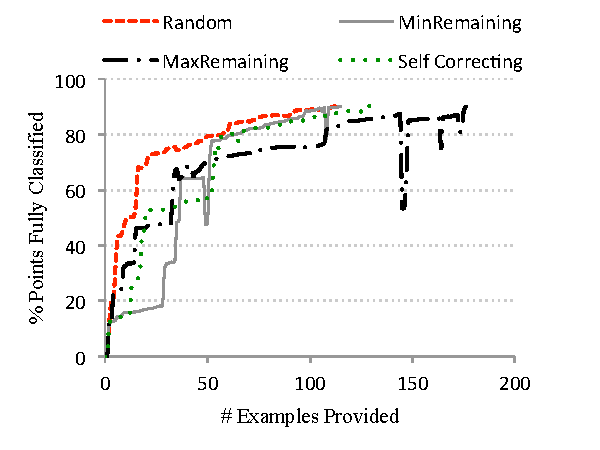
\includegraphics[width=\textwidth]{./figs/soda-active-learning.pdf}
                \caption{Building 1}
                \label{fig:active-learning-soda}
	\end{subfigure}
	\begin{subfigure}{0.48\textwidth}
                \centering
		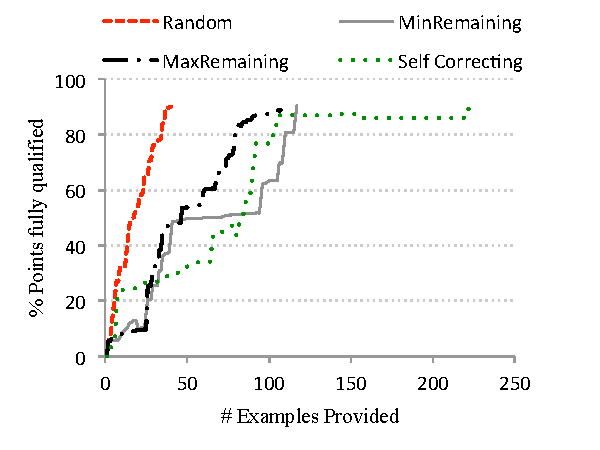
\includegraphics[width=\textwidth]{./figs/sdh-active-learning.pdf}
                \caption{Building 2}
                \label{fig:active-learning-sdh}
	\end{subfigure}
\caption{The number of examples required to fully qualify 70\% of sensor names in two buildings}
\label{fig:active-learning}
\end{figure}



\subsection{applying to other buildings}







